\lecture{6}

Roughly speaking, a topological manifold is a topological space that locally looks like \(\R^d\) for some fixed \(d \in \N\). For example, 2-sphere is a topological manifold as well as a 2-torus and a pretzel with \(d = 2\) in each case.

\section{Definition and Construction of Topological Manifolds}

\begin{definition}[Topological Manifold]
	A paracompact Hausdorff topological space \((M, \O)\) is called a \emph{d-dimensional (topological) manifold} if for every \(p \in M\) there exists an open neighborhood \(U_p \in \O\) of \(p\) and a homeomorphism \(x: U_p \to x(U_p) \subseteq \R^d\). And we write \(\dim{M} = d\).
\end{definition}

\begin{example}
	Let's go through some known topological spaces to see if they are topological manifolds.
	\begin{enumerate}
		\item Trivially, \(\R^d\) is a \(d\)-dimensional topological manifold for all \(d \ge 1\).
		\item The 1-sphere \(S^1\) is a 1-dimensional topological manifold.
		\item The topological spaces \(S^2\), \(C\) and \(T^2\) are 2-dimensional topological manifolds.
	\end{enumerate}
\end{example}

\begin{remark}[Local Homeomorphisms vs. Homeomorphisms]
	The definition of a topological manifold requires only local homeomorphisms. It is not necessary for the whole space to be homeomorphic to \(\R^d\). \\
	For example, the 1-sphere \(S^1\) is a 1-dimensional topological manifold, but it is not topologically isomorphic to \(\R\).
\end{remark}

\subsection{Submanifolds}

\begin{definition}[Submanifold]
	Let \((M, \O)\) be a topological manifold and \(N \subseteq M\) be a subset. Then \((N, \eval{\O}_N)\) is called a \emph{submanifold} of \((M, \O)\) if it is a topological manifold in its own right.
\end{definition}

\begin{example}
	The manifold \(S^1\) is a submanifold of \(\R^2\) while the manifolds \(S^2\), \(C\) and \(T^2\) are submanifolds of \(\R^3\).
\end{example}
Counterexample: The figure-eight curve is not a submanifold of \(\R^2\). As at the intersection point, we can't define dimension.

\begin{figure}[H]
	\centering
	\begin{subfigure}{0.4\textwidth}
		\centering
		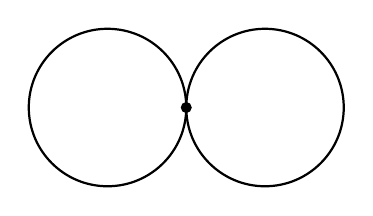
\begin{tikzpicture}
			\draw[thick] (-1,0) circle (1);
			\draw[thick] (1,0) circle (1);
			\fill (0, 0) circle (0.07);
		\end{tikzpicture}
		\caption{Figure-Eight in \(\R^2\)}
		\label{fig:figure-eight}
	\end{subfigure}
	\begin{subfigure}{0.4\textwidth}
		\centering
		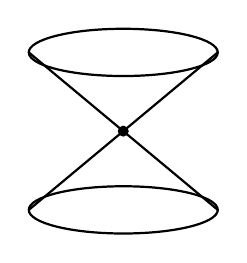
\begin{tikzpicture}
			\draw[thick] (0,1) ellipse (1.2 and 0.3);
			\draw[thick] (0,-1) ellipse (1.2 and 0.3);
			\draw[thick] (-1.2, 1) -- (1.2, -1);
			\draw[thick] (1.2, 1) -- (-1.2, -1);
			\fill (0, 0) circle (0.07);
		\end{tikzpicture}
		\caption{Light-Cone in Minkowski Spacetime}
		\label{fig:light-cone}
	\end{subfigure}
	\caption{Non-Submanifolds}
	\label{fig:non-submanifolds}
\end{figure}

We can see this in case of light-cone in Minkowski spacetime as well. The light-cone is also not a submanifold of Minkowski spacetime.

\subsection{Product Manifolds}

\begin{definition}[Product Manifold]
	Let \((M, \O_M)\) and \((N, \O_N)\) be topological manifolds. Then \((M \times N, \O_{M \times N})\) is a topological manifold called the \emph{product manifold} with \(\dim(M \times N) = \dim{M} + \dim{N}\).
\end{definition}

\begin{example}
	This shows that \(T^2 = S^1 \times S^1\) is a topological manifold of dimension 2. And we can generalize this to define \emph{\(n\)-torus} as
	\begin{equation}
		T^n := \underbrace{S^1 \times \cdots \times S^1}_{n\ \text{times}}
	\end{equation}
	which is a topological manifold of dimension \(n\).
\end{example}

Products are very useful. Very often in physics one intuitively thinks of the product of two
manifolds as attaching a copy of the second manifold to each point of the first.

Counterexample: M\"obius strip is not a product manifold.
\begin{figure}[H]
	\centering
	\begin{subfigure}{0.4\textwidth}
		\centering
		\begin{tikzpicture}[
				decoration={markings, mark=at position 0.5 with {\arrow{latex}}},
				scale=1.3
			]
			\draw[postaction={decorate}, thick] (-1.5, -0.75) -- (-1.5, 0.75);
			\draw[thick] (-1.5, 0.75) -- (1.5, 0.75);
			\draw[postaction={decorate}, thick] (1.5, 0.75) -- (1.5, -0.75);
			\draw[thick] (1.5, -0.75) -- (-1.5, -0.75);
		\end{tikzpicture}
		\caption{M\"obius Strip (easy to draw)}
		\label{fig:moebius-strip}
	\end{subfigure}
	\begin{subfigure}{0.4\textwidth}
		\centering
		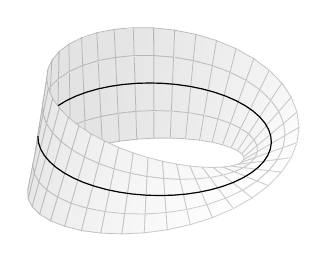
\begin{tikzpicture}[scale=0.7]
			\begin{axis}[
					hide axis,
					view={40}{45}
				]
				\addplot3 [
					surf, shader=faceted interp,
					point meta=x,
					colormap={slategraywhite}{rgb=(0.89,0.89,0.89) rgb=(1,1,1)},
					samples=40,
					samples y=5,
					%z buffer=sort,
					domain=0:360,
					y domain=-0.5:0.5
				] (
				{(1+0.5*y*cos(x/2)))*cos(x)},
				{(1+0.5*y*cos(x/2)))*sin(x)},
				{0.5*y*sin(x/2)});

				\addplot3 [
					samples=50,
					domain=-142:184.5, % The domain needs to be adjusted manually, depending on the camera angle, unfortunately
					samples y=0,
					semithick
				] (
				{cos(x)},
				{sin(x)},
				{0});
			\end{axis}
		\end{tikzpicture}
		\caption{M\"obius Strip (hard to draw)}
	\end{subfigure}
	\caption{Non-Product Manifolds}
	\label{fig:non-product-manifolds}
\end{figure}

\section{Bundles}

\begin{definition}[Bundle]\label{def:bundle}
	A \emph{bundle} (of a topological space) is a triple \((E, \pi, M)\) where \(E\) and \(M\) are topological spaces called the \emph{total space} and the \emph{base space} respectively, and \(\pi: E \to M\) is a continuous surjective map called the \emph{projection map}. \\
	We often denote the bundle as
	\begin{equation}
		\begin{tikzcd}
			E \arrow[r, "\pi"] & M
		\end{tikzcd}
	\end{equation}
\end{definition}

\begin{definition}[Fibre]\label{def:fibre}
	Let \((E, \pi, M)\) be a bundle and \(p \in M\). Then the set \(F_p := \preimg_{\pi}(\qty{p})\) is called the \emph{fibre} over \(p\).
\end{definition}

\begin{example}[Product Bundle]
	Let \(M\) and \(F\) be topological spaces. Define the product space \(E := M \times F\) and the projection map \(\pi: E \to M\) as \(\pi(m, f) = m\). Then \((E, \pi, M)\) is a bundle called the \emph{product bundle}. \\
	Define \(\pi': E \to F\) as \(\pi'(m, f) = f\). Then \((E, \pi', F)\) is also a product bundle.
\end{example}

\begin{example}[Mobius Strip as a Bundle]
	Consider the M\"obius strip as a bundle. Define the total space \(E\) as the M\"obius strip and the projection map \(\pi: E \to S^1\) as the projection of the M\"obius strip onto the circle. Then \((E, \pi, S^1)\) is a bundle.

	It is easy to see that the fibre over any point \(p \in S^1\) is a line segment. See \cref{fig:moebius-strip-bundle}.
	\begin{equation}
		\forall p \in S^1: F_p = [-1, 1]
	\end{equation}
	\begin{figure}[H]
		\centering
		\begin{tikzpicture}[
				decoration={markings, mark=at position 0.5 with {\arrow{latex}}},
				scale=2
			]
			\draw[thick, postaction={decorate}] (-1.5, -0.75) -- (-1.5, 0.75) node[left, scale=1] {1} node[left, pos=0, scale=1] {-1};
			\draw[thick] (-1.5, 0.75) -- (1.5, 0.75) node[right, scale=1] {\(E\)};
			\draw[thick, postaction={decorate}] (1.5, 0.75) -- (1.5, -0.75);
			\draw[thick] (1.5, -0.75) -- (-1.5, -0.75);
			\draw[gray, dashed] (-1.5, 0) -- (1.5, 0) node[right, scale=1] {\(S^1\)};
			\draw[blue, <<->>] (-0.7, 0.75) -- (-0.7, -0.75) node[pos = 0.8, right, scale=1] {\(F_p\)};
			\fill (-0.7, 0) circle (0.03) node[above left, scale=1] {\(p\)};
			\fill (0.7, 0.4) circle (0.03) node[above right, scale=1] {\(q\)};
			\draw[red, ->] (0.7, 0.4) -- (0.7, 0) node[pos = 0.5, right, scale=1] {\(\pi\)};
			\fill[red] (0.7, 0) circle (0.03);
		\end{tikzpicture}
		\caption{M\"obius Strip as a Bundle}
		\label{fig:moebius-strip-bundle}
	\end{figure}
\end{example}

In both the examples, the fibre over any point in the base space is the same. But this is not necessary. The fibre can be different over different points in the base space.
\begin{example}
	Consider the base space \(M = \R\) and the total space as defined in \cref{fig:nontrivial-bundle}.
	\begin{figure}[H]
		\centering
		\begin{tikzpicture}[scale=1.25]
			\draw[thick, <->] (-4, 0) -- (4, 0);
			\fill (0, 0) circle (0.07) node[below] {\(0\)};
			\draw (-1, 0.45) circle (0.45) node[above] {\(S^1\)};
			\fill (-1, 0) circle (0.06) node[below] {\(-1\)};
			\draw[(-)] (1, 1) -- (1, -1) node[above, pos=0] {\(1\)} node[below] {\(-1\)};
			\fill (1, 0) circle (0.06) node[below right] {\(1\)};
			\draw (-2, 0.45) circle (0.45) node[above] {\(S^1\)};
			\fill (-2, 0) circle (0.06) node[below] {\(-2\)};
			\draw[(-)] (2, 1) -- (2, -1) node[above, pos=0] {\(1\)} node[below] {\(-1\)};
			\fill (2, 0) circle (0.06) node[below right] {\(2\)};
			\draw (-3, 0.45) circle (0.45) node[above] {\(S^1\)};
			\fill (-3, 0) circle (0.06) node[below] {\(-3\)};
			\draw[(-)] (3, 1) -- (3, -1) node[above, pos=0] {\(1\)} node[below] {\(-1\)};
			\fill (3, 0) circle (0.06) node[below right] {\(3\)};
		\end{tikzpicture}
		\caption{Total Space \(E\)}
		\label{fig:nontrivial-bundle}
	\end{figure}
	Here, the fibre over every point in the base space is not the same.
	\begin{equation}
		\forall p \in \R: F_p \topIso \begin{cases}
			S^1         & \text{if}\ p < 0 \\
			\qty{0}     & \text{if}\ p = 0 \\
			\qty(1, -1) & \text{if}\ p > 0
		\end{cases}
	\end{equation}
\end{example}

\subsection{Fibre Bundles}

\begin{definition}[Fibre Bundle]
	Let \(E \xrightarrow[]{\ \pi\ } M\) be a bundle. Then \((E, \pi, M)\) is called a \emph{fibre bundle} if
	\begin{equation}
		\exists F (=\text{topological space}): \forall p \in M: F_p \topIso F
	\end{equation}
\end{definition}
We can think of a fibre bundle as an attachment of a copy of the fibre \(F\) to each point of the base space \(M\). Notationally, we write
\begin{equation}
	\begin{tikzcd}
		F \arrow[r] & E \arrow[d, "\pi"] \\
		& M
	\end{tikzcd}
\end{equation}

It is easy to see that the product bundle is a fibre bundle. But the converse is not true.
\begin{example}[M\"obius Strip as a Fibre Bundle]
	Let M\"obius strip be our total space and 1-sphere \(S^1\) be our base space. Then the M\"obius strip is a fibre bundle over the 1-sphere with the typical fibre \([-1, 1]\). See \cref{fig:moebius-strip-bundle}.\\
	Keep in mind that \(E \ne S^1 \times [-1, 1]\) \ie\ M\"obius strip is not a product bundle.
\end{example}

\begin{example}[\(\C^1\)-line bundle]
	A \(\C\)-line bundle over \(M\) is the fibre bundle \((E,\pi,M)\) with fibre \(\C\). \\
	Note that \(M \times \C \xrightarrow[]{\ \pi\ } M\) is a \(\C\)-line bundle over \(M\), but a \(\C\)-line bundle over \(M\) need not be a product bundle.
\end{example}

\begin{definition}[Section]
	Let \(E \xrightarrow[]{\ \pi\ } M\) be a bundle. A map \(\sigma: M \to E\) is called a (\emph{cross}-)\emph{section} of the bundle if \(\pi \circ \sigma = \id_M\).
\end{definition}

Intuitively, a section is a map \(\sigma\) which sends each point \(p \in M\) to some point \(\sigma(p)\) in its fibre \(F_p\), so that the projection map \(\pi\) takes \(\sigma(p) \in F_p \subseteq E\) back to the point \(p \in M\).

\begin{example}[Special Case for Product Bundles]
	Let \(M \times F \xrightarrow[]{\ \pi\ } M\) be a product bundle. Let \(s: M \to F\) be a map. Then the map
	\begin{equation}
		\begin{aligned}
			\sigma: M & \to M \times F    \\
			p         & \mapsto (p, s(p))
		\end{aligned}
	\end{equation}
	is a section of the product bundle. \\
	Thus, for product bundles, sections are in one-to-one correspondence with maps \(M \to F\) \ie\ by choosing a map \(s: M \to F\), we get a section \(\sigma: M \to M \times F\).
\end{example}
In case of product bundles, we can analyze `section' of the bundle by looking at the corresponding map \(s: M \to F\).

\noindent With this we can order the bundles as follows:
\begin{equation}
	\text{Product Bundles} \subset \text{Fibre Bundles} \subset \text{Bundles}
\end{equation}

At this point, we can have a physics example (from quantum mechanics) but to understand it fully, we require more maturity.
\begin{example}[Wave functions]
	Consider our base space \(M\) to be our physical space (for case \(\R^3\)). The mathematical structure, we are analyzing in quantum mechanics is \(\C^1\)-line bundle over physical space.
	\begin{equation}
		\text{wave function} := \text{section of \((E, \pi, M)\)}
	\end{equation}
	In case, \(E\) is a product manifold of \(M\) and \(\C\), then wave function is a function.
\end{example}

\subsection{Constructing Bundles}

\begin{definition}[Sub-Bundle]
	Let \(E \xrightarrow[]{\ \pi\ } M\) and \(E' \xrightarrow[]{\ \pi'\ } M'\) be bundles. Then \((E', \pi', M')\) is called a \emph{sub-bundle} of \((E, \pi, M)\) if
	\begin{enumerate}
		\item \(E' \subseteq E\) be a submanifold,
		\item \(M' \subseteq M\) be a submanifold, and
		\item \(\pi' = \eval{\pi}_{E'}\).
	\end{enumerate}
\end{definition}

\begin{definition}[Restricted Bundle]
	Let \(E \xrightarrow[]{\ \pi\ } M\) be a bundle and \(N \subseteq M\) be a submanifold. Then the bundle
	\begin{equation}
		\preimg_{\pi}(N) \xrightarrow[]{\ \eval{\pi}_{\preimg_{\pi}(N)}\ } N
	\end{equation}
	is called the \emph{restricted bundle} of \((E, \pi, M)\) to \(N\).
\end{definition}

\section{Bundle Morphisms}

\begin{definition}[Bundle Morphism]\label{def:bundle-morphism}
	Let \(E \xrightarrow[]{\ \pi\ } M\) and \(E' \xrightarrow[]{\ \pi'\ } M'\) be bundles and \(u: E \to E'\) and \(v: M \to M'\) be continuous maps. Then \((u, v)\) is called a \emph{bundle morphism} if
	\begin{equation}
		\begin{tikzcd}
			E \arrow[r, "u"] \arrow[d, "\pi"'] & E' \arrow[d, "\pi'"] \\
			M \arrow[r, "v"']                  & M'
		\end{tikzcd}
	\end{equation}
	commutes \ie\ \(\pi' \circ u = v \circ \pi\).
\end{definition}

\begin{definition}[Bundle Isomorphism]\label{def:bundle-isomorphism}
	Let \(E \xrightarrow[]{\ \pi\ } M\) and \(E' \xrightarrow[]{\ \pi'\ } M'\) be bundles. They are called \emph{isomorphic} (as bundles) if there exist bundle morphisms \((u, v)\) such that
	\begin{equation}
		\begin{tikzcd}
			E \arrow[rr,shift left,"u"] \arrow[dd,"\pi"'] & & E' \arrow[ll,shift left,"u^{-1}"] \arrow[dd,"\pi'"] \\
			& & \\
			M \arrow[rr,shift left,"v"] & & M' \arrow[ll,shift left,"v^{-1}"]
		\end{tikzcd}
	\end{equation}
	is a commutative diagram. Such a bundle morphism \((u, v)\) is called a \emph{bundle isomorphism}. And we write \(E \xrightarrow[]{\ \pi\ } M \bdlIso E' \xrightarrow[]{\ \pi'\ } M'\).
\end{definition}

Bundle isomorphisms are structure-preserving maps between bundles.

\begin{definition}[Local Isomorphism]
	Let \(E \xrightarrow[]{\ \pi\ } M\) and \(E' \xrightarrow[]{\ \pi'\ } M'\) be bundles. Then \(E \xrightarrow[]{\ \pi\ } M\) is called \emph{locally isomorphic} to \(E' \xrightarrow[]{\ \pi'\ } M'\) if
	\begin{equation}
		\forall p \in M: \exists U_p \in \O_M: \preimg_{\pi}(U_p) \xrightarrow[]{\ \eval{\pi}_{\preimg_{\pi}(U_p)}\ } U_p \bdlIso E' \xrightarrow[]{\ \pi'\ } M'.
	\end{equation}
\end{definition}

\noindent Some useful terminologies:
\begin{definition}
	A bundle \(E \xrightarrow[]{\ \pi\ } M\) is called
	\begin{enumerate}[(a)]
		\item \emph{trivial} if it is isomorphic to a product bundle \(M \times F \xrightarrow[]{\ \pi_1\ } M\).
		\item \emph{locally trivial} if it is locally isomorphic to some product bundle.
	\end{enumerate}
\end{definition}
It is obvious that every trivial bundle is locally trivial. But the converse is not true.

\begin{example}
	Let's see some insightful examples:
	\begin{enumerate}
		\item A cylinder \(C\) is trivial \(\implies\) locally trivial.
		\item M\"obius Strip is not trivial, but it is locally trivial.
		\item A very specific construction, such that the bundle is not even locally trivial.
		      \begin{figure}[H]
			      \centering
			      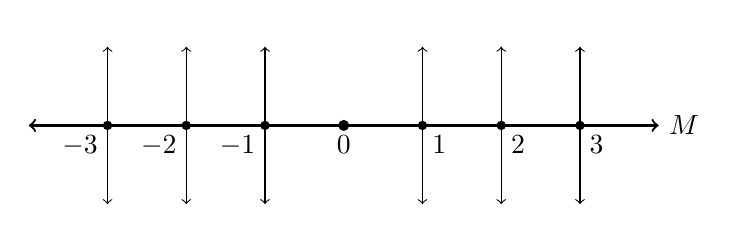
\begin{tikzpicture}[scale=1]
				      \draw[thick, <->] (-4, 0) -- (4, 0) node[right] {\(M\)};
				      \fill (0, 0) circle (0.07) node[below] {\(0\)};
				      \draw[<->] (-1, -1) -- (-1, 1) node[above] {\(\C\)};
				      \fill (-1, 0) circle (0.06) node[below left] {\(-1\)};
				      \draw[<->] (1, 1) -- (1, -1) node[below] {\(\R\)};
				      \fill (1, 0) circle (0.06) node[below right] {\(1\)};
				      \draw[<->] (-2, -1) -- (-2, 1) node[above] {\(\C\)};
				      \fill (-2, 0) circle (0.06) node[below left] {\(-2\)};
				      \draw[<->] (2, 1) -- (2, -1) node[below] {\(\R\)};
				      \fill (2, 0) circle (0.06) node[below right] {\(2\)};
				      \draw[<->] (-3, -1) -- (-3, 1) node[above] {\(\C\)};
				      \fill (-3, 0) circle (0.06) node[below left] {\(-3\)};
				      \draw[<->] (3, 1) -- (3, -1) node[below] {\(\R\)};
				      \fill (3, 0) circle (0.06) node[below right] {\(3\)};
			      \end{tikzpicture}
			      \caption{Non Locally Trivial bundle}
			      \label{fig:nonlocaltrivial-bundle}
		      \end{figure}
	\end{enumerate}
\end{example}
From now on, we will be focusing on locally trivial bundles unless mentioned otherwise.

\begin{remark}
	Since we have restricted ourselves to locally trivial bundles. Thus, any section can be thought of as a map \(M \to F\) locally.
\end{remark}

\begin{example}[Wave functions (revisited)]
	Assume that our \(\C^1\)-line bundle over \(M (= \R^3)\) is locally trivial. Then the wave function is a function \(M \to \C\) locally.
\end{example}

\begin{definition}[Pull-Back Bundle]
	Let \(E \xrightarrow[]{\ \pi\ } M\) be a bundle and \(f: M' \to M\) be a map from another manifold \(M'\) to \(M\). Define the manifold \(E'\) as
	\begin{equation}
		E' := \qty{(m', e) \in M' \times E \mid f(m') = \pi(e)}.
	\end{equation}
	Then the bundle \((E', \pi', M')\) with \(\pi'(m', e) = m'\) is called the \emph{pull-back bundle} of \(E \xrightarrow[]{\ \pi\ } M\) induced by \(f: M' \to M\).
\end{definition}

\begin{remark}[Bundle Morphism on Pull-Back Bundle]
	Let \(E' \xrightarrow[]{\ \pi'\ } M'\) be a pull-back bundle of \(E \xrightarrow[]{\ \pi\ } M\) induced by \(v: M' \to M\). Define the map
	\begin{equation}
		\begin{aligned}
			u: E'   & \to E      \\
			(m', e) & \mapsto e.
		\end{aligned}
	\end{equation}
	Then \((u, v)\) is a bundle morphism. This corresponds to the commutative diagram
	\begin{equation*}
		\begin{tikzcd}
			E' \arrow[r, "u"] \arrow[d, "\pi'"'] & E \arrow[d, "\pi"] \\
			M' \arrow[r, "v"']                    & M
		\end{tikzcd}
	\end{equation*}
\end{remark}

\begin{remark}[Pull-back of Sections]
	Let \(E' \xrightarrow[]{\ \pi'\ } M'\) be a pull-back bundle of \(E \xrightarrow[]{\ \pi\ } M\) induced by \(f: M' \to M\). Let \(\sigma\) be a section of \(E \xrightarrow[]{\ \pi\ } M\).
	\begin{equation*}
		\begin{tikzcd}
			E' \arrow[dd, shift left, "\pi'"] & & E \arrow[dd, shift left, "\pi"] \\
			& & \\
			M' \arrow[uu, blue, shift left, "\sigma'"] \arrow[rr, "f"] \arrow[rruu, purple, "\sigma \circ f"] & & M \arrow[uu, shift left, "\sigma"]
		\end{tikzcd}
	\end{equation*}
	Observe that \(\sigma \circ f\) is a map \(M' \to E\). Using the fact that \(\sigma\) is a section, we have,
	\begin{gather}
		(\pi \circ (\sigma \circ f))(m') = ((\pi \circ \sigma) \circ f)(m') = (\id_{M} \circ f)(m') = f(m') \nonumber \\
		\intertext{This can be interpreted as \(\pi((\sigma \circ f)(m')) = f(m')\). Thus, \((m', (\sigma \circ f)(m')) \in E'\). Define the map \(\sigma'\) as}
		\begin{aligned}
			\sigma': M' & \to E'                              \\
			m'          & \mapsto (m', (\sigma \circ f)(m')).
		\end{aligned}
	\end{gather}
	Furthermore, \(\pi' \circ \sigma' = \id_{M'}\) as \(\pi'(m', (\sigma \circ f)(m')) = m'\). Thus, \(\sigma'\) is a section of the pull-back bundle.
\end{remark}

\section{Viewing Manifolds from Atlases}

\begin{definition}[Chart]\label{def:chart}
	Let \((M, \O)\) be a \(d\)-dimensional manifold. Then the pair \((U, x)\), where \(U \in \O\) and \(x: U \to x(U) \subseteq \R^d\) is a homeomorphism, is called a \emph{chart} on \(M\).
\end{definition}

\begin{remark}[Component Functions]\label{rem:component-functions}
	Let \((U, x)\) be a chart on \(M\). Then the \emph{component functions} of \(x\) are the functions
	\begin{equation}
		\begin{aligned}
			x^i: U & \to \R                \\
			p      & \mapsto \proj_i(x(p))
		\end{aligned}
	\end{equation}
	for \(1 \le i \le d\), where \(\proj_i\) is the \(i\)-component of \(x(p) \in \R^d\). The \(x^i(p)\)'s are called \emph{co-ordinate} of the point \(p \in U\) with respect to the chart \((U, x)\).
\end{remark}

\begin{definition}[Atlas]\label{def:atlas}
	Let \((M, \O)\) be a \(d\)-dimensional manifold. Then the collection of all charts \(\mathscr{A} := \qty{(U_\alpha, x_\alpha) \mid \alpha \in I}\) is called an \emph{atlas} of the manifold \(M\) if,
	\begin{equation}
		\bigcup_{\alpha \in I} U_\alpha = M,
	\end{equation}
	for some index set \(I\).
\end{definition}

This is obvious to see that this collection is a set, as from the definition of manifolds, we have an open set \(U_p\) at each point with an appropriate homeomorphism \(x_p\). Thus, this provides a trivial atlas of \(M\),
\begin{equation}
	\mathscr{A} = \qty{(U_p, x_p) \mid p \in M}
\end{equation}

\begin{definition}[\(\SC^0\)-Compatibility]
	Let \((U_\alpha, x_\alpha)\) and \((U_\beta, x_\beta)\) be two charts of a manifold \(M\). They are called \emph{\(\SC^0\)-compatible} either
	\begin{enumerate}[(a)]
		\item \(U_\alpha \cap U_\beta = \0\), or
		\item the map \(x_{\beta} \circ x_{\alpha}\inv: x_{\alpha}(U_{\alpha} \cap U_{\beta}) \to x_{\beta}(U_{\alpha} \cap U_{\beta})\) is continuous.
	\end{enumerate}
\end{definition}

\(x_{\beta} \circ x_{\alpha}\inv\) (and its inverse \(x_{\alpha} \circ x_{\beta}\inv\)) is a map from a subset of \(\R^d\) to another subset of \(\R^d\).
\begin{figure}[H]
	\centering
	\begin{tikzcd}
		& U_{\alpha} \cap U_{\beta} \arrow[ld, "x_{\alpha}"'] \arrow[rd, "x_{\beta}"] & \\
		\R^d \supseteq x_{\alpha}(U_{\alpha} \cap U_{\beta}) \arrow[rr, shift left, "x_{\beta} \circ x_{\alpha}\inv"] & & x_{\beta}(U_{\alpha} \cap U_{\beta}) \subseteq \R^d \arrow[ll, shift left, "x_{\alpha} \circ x_{\beta}\inv"]
	\end{tikzcd}
\end{figure} \noindent

Here it may seem like a redundant definition, since \(x_{\alpha}\) and \(x_{\beta}\) are homeomorphisms, the composition map \(x_{\beta} \circ x_{\alpha}\inv\) (or its inverse \(x_{\alpha} \circ x_{\beta}\inv\)) is also a homeomorphism thus continuous. Therefore, any two charts on a topological manifold are \(\SC^0\)-compatible.

This notion will be useful, when we want to talk about differentialable manifolds. In that case, we require the map \(x_{\beta} \circ x_{\alpha}\inv\) to be continuously differentiable or \(k\)-smooth for \(\SC^1\) or \(\SC^k\)-compatible respectively using the notion of differentiability on \(\R^d\).

\begin{remark}[Co-ordinate Change]
	The map \(\tau_{\alpha, \beta} := x_{\beta} \circ x_{\alpha}\inv\) (and its inverse \(\tau_{\beta, \alpha} := x_{\alpha} \circ x_{\beta}\inv\)) is called the \emph{co-ordinate change map} or \emph{chart transition map}.
\end{remark}
This also express that, all the physics that we have done so far lives in chart. For example, the motion of a particle is a subset of our physical manifold, and we use different co-ordinates (or charts) for our understanding.

\begin{definition}[\(\SC^0\)-Atlas]
	An atlas \(\mathscr{A}\) is a \emph{\(\SC^0\)-atlas} if all the charts in \(\mathscr{A}\) are pairwise \(\SC^0\)-compatible.
\end{definition}

\noindent Any atlas is a \(\SC^0\)-atlas.

\begin{definition}[Maximal Atlas]
	A \(\SC^0\)-atlas \(\mathscr{A}\) is called a \emph{maximal} if it contains every chart that is \(\SC^0\)-compatible with every chart in \(\mathscr{A}\).
\end{definition}

\begin{example}
	Let \((\R, \Ostd)\) be our topological manifold. Then we have a trivial atlas \(\mathscr{A} = \qty{(\R, \id_{\R})}\), but it is not maximal. Since chart \(((0, 1), \id_{(0, 1)})\) is \(\SC^0\)-compatible with the chart \((\R, \id_{\R})\), but it is not in the atlas \(\mathscr{A}\).
\end{example}

We can look at ``objects on'' topological manifolds from two point of view. Consider a curve \(\gamma\) in a \(d\)-dimensional manifold, \ie\ \(\gamma: \R \to M\). From our previous knowledge, we know this curve has to be continuous if it describes the trajectory of a classical particle.

One way to verify this, let an open set in \(M\) and check whether its pre-image is open or not (topological definition).

Another way is through the concept of charts. Let \((U, x)\) be a chart, rather than studying \(\gamma\) directly, we will focus on \(x \circ \gamma: \R \supseteq \preimg_{\gamma}(U) \to x(U) \subseteq \R^d\). Checking continuity of this composition map is easier as well as guarantees the continuity of \(\gamma\).

Let the problem is very complicated in this co-ordinate system, let \((U, y)\) be another chart. And this change of co-ordinate is facilitated by transition maps. We can summarize all this in the following cummatative diagram:
\begin{figure}[H]
	\centering
	\begin{tikzcd}
		&& y(U) \subseteq \R^d \arrow[dddd, bend left=110, shift left, "x \circ y\inv"] \\
		&&\\
		\preimg_{\gamma}(U) \subseteq \R \arrow[rr, "{\gamma}"] \arrow[ddrr, "x \circ {\gamma}"'] \arrow[uurr, "y \circ {\gamma}"]&& U \subseteq M \arrow[dd, "x"] \arrow[uu, "y"'] \\
		&&\\
		&& x(U) \subseteq \R^d \arrow[uuuu, bend right=75, shift left, "y \circ x\inv"]
	\end{tikzcd}
	\caption{Looking at Continuity of a curve in a manifold using charts}
	\label{fig:chart_application_curves}
\end{figure}

Intuitively, this description allows us to forget about the inner structure (\ie\ \(U\) and the maps \(\gamma\), \(x\) and \(y\)) which, in a sense, is the real world, and only consider \(\preimg_{\gamma}(U) \subseteq \R\) and \(x(U), y(U) \subseteq \R^d\) together with the maps between them, which is our representation of the real world.
